\section{Territory}
\begin{itemize}
    \item Territory is an essential element of statehood; it is within territory that a state's legal authority is exercised
    \item Sovereignty in relation to territory is ``the right to exercise therein, to the exclusion of any other State, the functions of a State'' -- \case{\textit{Island of Palmas} (1928)}
    \item ``The basic legal concept of State sovereignty in customary international law, expressed in ... Art 2(1), of the UN Charter, extends to the internal waters and territorial sea of every State and to the air space above its territory'' -- \case{\textit{Nicaragua} [1986] ICJ Rep 14}
    \item There is a distinction between sovereignty (dominium) and jurisdiction (imperium)
\end{itemize}

\section{Modes of Acquiring Territory}
\subsection{Occupation}
\begin{itemize}
    \item Occupation is the formal act of intention and demonstration of effective control over territory
    \item Territory may be acquired through occupation if it is \textit{terra nullius} (i.e., no population, or if the territory is abandoned)
    \item Occupation is ``an original means of peaceably acquiring sovereignty over territory'' -- \case{\textit{Western Sahara Advisory Opinion} [1975] ICJ Rep 162}
\end{itemize}

\begin{casedetails}{\textit{Western Sahara Advisory Opinion} [1975] ICJ Rep 162}
    \flushleft
    This case concerned a dispute over sovereignty to West Sahara, which was formerly a Spanish colony. It was claimed by both Morocco (on the basis of Spain's former colonisation), and by Mauritania. 

    \vspace{\baselineskip}

    \textbf{To be completed from lecture notes.}
\end{casedetails}

\begin{casedetails}{\textit{Mabo v Queensland (No 2)} (1992) 175 CLR 1}
    \flushleft
    \textbf{To be completed from lecture notes.}
\end{casedetails}

\begin{itemize}
    \item For an intention to occupy to be manifest:
    \begin{itemize}
        \item There must be an expression of formal intent to claim possession of the land (e.g., the planting of a flag); this is known as \textit{animus occupandi}
        \item Territory must be claimed by a state authority, not a private actor
    \end{itemize}
    \item Under Australian law, individuals may not acquire title in unoccupied land not claimed by a state, following \case{\textit{Ure v Commonwealth} [2016] FCAFC 8} (Page \pageref{case:Ure v Commonwealth})
    \item For there to be effective occupation, there must be:
    \begin{itemize}
        \item A continuous and peaceful display of state authority
        \item A responsible authority that exercises governmental functions (\textit{effectivités})
        \item Spatial extent (although not necessarily all territory), duration, continuity, and peacefulness are all relevant considerations
    \end{itemize}
\end{itemize}

\begin{casedetails}{\textit{Clipperton Island Arbitration (France v Mexico)} 1932}
    \flushleft
    \textbf{To be completed from lecture notes.}
\end{casedetails}

\subsection{Cession}
\begin{itemize}
    \item Cession is the intentional transfer of sovereignty over territory from one state to another
\end{itemize}

\subsection{Prescription}
\begin{itemize}
    \item Prescription is the acquisition of title to territory formerly occupied by another state through a peaceful exercise of sovereignty
\end{itemize}

\begin{casedetails}{\textit{Island of Palmas Case (Netherlands v US)} (1928)}
    \flushleft
    \textbf{To be completed from lecture noted.}
\end{casedetails}

\subsection{Accretion and Avulsion}
\begin{itemize}
    \item Accretion is the gain of physical territory through natural processes
    \item Avulsion is the loss of physical territory through natural processes
\end{itemize}

\subsection{Conquest}
\begin{itemize}
    \item Conquest is the forceful, unlawful acquisition of territory
    \item Under \convention{\textit{Charter of the United Nations} Art 2(4)}, conquest is now illegal under international law
\end{itemize}

\section{Contested Territorial Sovereignty}
\begin{casedetails}{\textit{Legal Status of Eastern Greenland (Norway v Denmark)} (1933) PCIJ}
    \flushleft
    \textbf{To be completed from lecture notes.}
\end{casedetails}

\begin{casedetails}{\textit{Case Concerning Sovereignty Over Pulau Ligitan and Pulau Spiadan (Indonesia v Malaysia)} [2002] ICJ Rep 625}
    \flushleft
    \textbf{To be completed from lecture notes.}
\end{casedetails}

\begin{casedetails}{\textit{Case Concerning Sovereignty Over Pedra Branca/Pulau Batu Puteh, Middle Rocks and South Ledge (Malaysia/Singapore)} [2008] ICJ Rep 12}
    \flushleft
    \textbf{To be completed from lecture notes.}
\end{casedetails}

\section{Maritime Zones}
\begin{itemize}
    \item Maritime zones are governed by the \convention{\textit{1982 UN Convention on the Law of the Seas} (UNCLOS)}
\end{itemize}

\begin{figure}[H]
    \centering
    \includegraphics[width=1\textwidth]{Images/Maritime Zones.png}
    \caption{Maritime Zones as Defined in the UNCLOS}
    \label{fig:Maritime Zones}
\end{figure}

\begin{figure}[H]
    \centering
    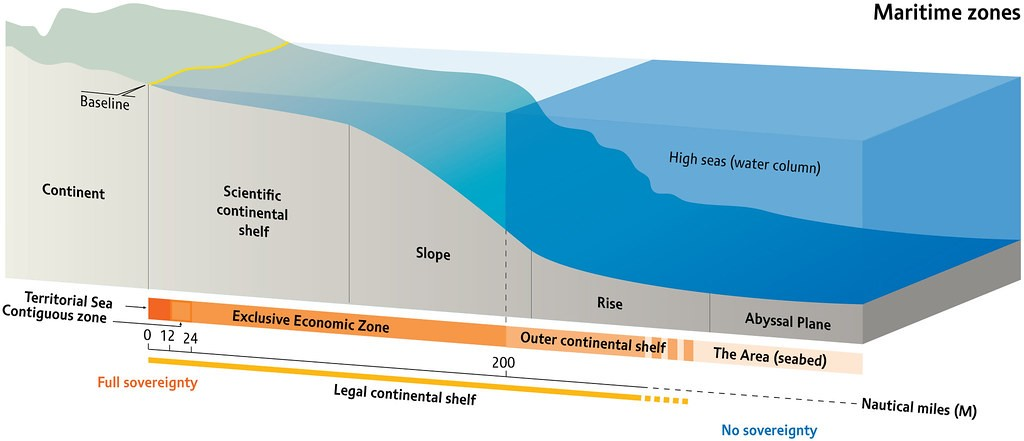
\includegraphics[width=1\textwidth]{Images/UNCLOS Maritime Zones.jpeg}
    \caption{Maritime Zones as Defined in the UNCLOS (Alternative Representation)}
    \label{fig:UNCLOS Maritime Zones}
\end{figure}

\begin{casedetails}{\textit{South China Sea Arbitration (Philippines v China)} [2016] PCA}
    \flushleft
    \textbf{To be completed from lecture notes.}
\end{casedetails}

\section{Antarctica}
\begin{itemize}
    \item There are 7 claimants to territory in Antarctica: Argentina, Australia, Chile, France, New Zealand, Norway, and the UK
    \item Article 4 of the \convention{\textit{1959 Antarctic Treaty}} provides that no new claims to territory in Antarctica may be made, but that there is no renunciation of any existing claims (i.e., they are frozen whilst the treaty is in force)
    \item Whilst the treaty is in force, no acts conducted can constitute a basis for asserting, supporting or denying a claim to territorial sovereignty in Antarctica
\end{itemize}

\begin{conventiondetails}{\textit{1959 Antarctic Treaty} Art 4}
    \flushleft 
    \begin{enumerate}
        \item Nothing contained in the present Treaty shall be interpreted as:
        \begin{enumerate}[label=(\alph*)]
            \item a renunciation by any Contracting Party of previously asserted rights of or claims to territorial sovereignty in Antarctica;
            \item a renunciation or diminution by any Contracting Party of any basis of claim to territorial sovereignty in Antarctica which it may have whether as a result of its activities or those of its nationals in Antarctica, or otherwise;
            \item prejudicing the position of any Contracting Party as regards its recognition or non-recognition of any other State’s right of or claim or basis of claim to territorial sovereignty in Antarctica.
        \end{enumerate}
        \item No acts or activities taking place while the present Treaty is in force shall 
        constitute a basis for asserting, supporting or denying a claim to territorial 
        sovereignty in Antarctica or create any rights of sovereignty in Antarctica. No new 
        claim, or enlargement of an existing claim, to territorial sovereignty in Antarctica 
        shall be asserted while the present Treaty is in force.
    \end{enumerate}
\end{conventiondetails}

\section{Airspace and Outer Space}

\subsection{Airspace}
\begin{itemize}
    \item A state has sovereignty over the airspace above its territory and territorial sea (\textit{cujus est solum ejus est usque ad coelum})
    \item Other states have the freedom of overflight over the contiguous zone, the EEZ, and high seas
    \item The boundary between national airspace and outer space is not clearly defined
\end{itemize}

\subsection{Outer Space}
\begin{itemize}
    \item The \convention{\textit{1967 Outer Space Treaty} Art 2} provides that outer space is not subject to national appropriation by any means
    \item Article 1 of this treaty additionally holds that outer space is the province of mankind
    \item There are 113 parties to this treaty
\end{itemize}

\begin{conventiondetails}{\textit{1967 Outer Space Treaty}}
    \flushleft
    \tcbsubtitle{Article 1}
    The exploration and use of outer space, including the moon and other celestial bodies, shall be carried out for the benefit and in the interests of all countries, irrespective of their degree of economic or scientific development, and shall be the province of all mankind.

    \vspace{\baselineskip}
    
    Outer space, including the moon and other celestial bodies, shall be free for exploration and use by all States without discrimination of any kind, on a basis of equality and in accordance with international law, and there shall be free access to all areas of celestial bodies.

    \vspace{\baselineskip}
    
    There shall be freedom of scientific investigation in outer space, including the moon and other celestial bodies, and States shall facilitate and encourage international co-operation in such investigation.
    \tcbsubtitle{Article 2}
    Outer space, including the moon and other celestial bodies, is not subject to national appropriation by claim of sovereignty, by means of use or occupation, or by any other means.
\end{conventiondetails}

\begin{itemize}
    \item The \convention{\textit{1979 Moon Agreement} Art 11(1)} provides that the moon and other celestial bodies are the common heritage of mankind
    \item There are only 18 parties to this treaty
\end{itemize}

\begin{conventiondetails}{\textit{1979 Agreement Governing the Activities of States on the Moon and Other Celestial Bodies}}
    \flushleft
    \tcbsubtitle{Article 11}
    \begin{enumerate}
        \item The moon and its natural resources are the common heritage of mankind, which finds its expression in the provisions of this Agreement, in particular in paragraph 5 of this article.
        \item The moon is not subject to national appropriation by any claim of sovereignty, by means of use or occupation, or by any other means.
        \item Neither the surface nor the subsurface of the moon, nor any part thereof or natural resources in place, shall become property of any State, international intergovernmental or non- governmental organization, national organization or non-governmental entity or of any natural person. The placement of personnel, space vehicles, equipment, facilities, stations and installations on or below the surface of the moon, including structures connected with its surface or subsurface, shall not create a right of ownership over the surface or the subsurface of the moon or any areas thereof. The foregoing provisions are without prejudice to the international regime referred to in paragraph 5 of this article.
        \item States Parties have the right to exploration and use of the moon without discrimination of any kind, on the basis of equality and in accordance with international law and the terms of this Agreement.
        \item States Parties to this Agreement hereby undertake to establish an international regime, including appropriate procedures, to govern the exploitation of the natural resources of the moon as such exploitation is about to become feasible. This provision shall be implemented in accordance with article 18 of this Agreement.
        \item In order to facilitate the establishment of the international regime referred to in paragraph 5 of this article, States Parties shall inform the Secretary-General of the United Nations as well as the public and the international scientific community, to the greatest extent feasible and practicable, of any natural resources they may discover on the moon.
        \item The main purposes of the international regime to be established shall include:
        \begin{enumerate}[label=(\alph*)]
            \item The orderly and safe development of the natural resources of the moon;
            \item The rational management of those resources;
            \item The expansion of opportunities in the use of those resources;
            \item An equitable sharing by all States Parties in the benefits derived from those resources, whereby the interests and needs of the developing countries, as well as the efforts of those countries which have contributed either directly or indirectly to the exploration of the moon, shall be given special consideration.
        \end{enumerate}
        \item All the activities with respect to the natural resources of the moon shall be carried out in a manner compatible with the purposes specified in paragraph 7 of this article and the provisions of article 6, paragraph 2, of this Agreement.
    \end{enumerate}
\end{conventiondetails}